\chapter{Compressive Sensing}

\section{The Compressive Sensing Problem}
\emph{
\begin{itemize}
\item Intro to CS. Outline main ideas
\item Conventional Sampling, Conversion
\item Problem Statement for discrete. Img, Vids as unrolled vec. Sparsity -> Compression (adaptive). Why wasteful.
\item CS is NON-ADAPTIVE. Sensing Matrix. Much fewer measurements.
\item Against Fund Thm of LA -> resolve by sparsity (show a graphic).
\item What Sensing matrix? We've only done masks, so maybe no point in talking about RIP etc -> just reference.
\item Signal Recovery. L2 vs L0 vs L1 + Geometry?.
\item We focus on Reconstruction. Side note to single-px cam (in \@ sensing). Perhaps this should go in Ch1:Background
\end{itemize}
}

This section is based on \cite{pilikos2014}. 
The problem to be solved can be formulated as follows: Let $\bs x \in \mathbb{R}^N$ be a signal of interest.
We do not measure $\bs x$ directly and it is thus unknown.
Instead, we have a measurement $\bs y \in \mathbb{R}^M$, with $M << N$, from which we want to reconstruct $\bs x$.
The signals $\bs x$ and $\bs y$ are related as follows:
\begin{equation}
\label{eqn:CS}
\bs \Omega \bs x = \bs y
\end{equation}
where $\bs \Omega$ is a known $M\times N$ matrix referred to as the \emph{sensing matrix}.

\begin{figure}
\caption{Example of a signal pair $\bs x$ (left) and $\bs y$ (right). We wish to reconstruct $\bs x$ from $\bs y$.}
\label{fig:lenna}
\center

\includegraphics{Images/128.png}
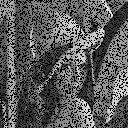
\includegraphics{Images/0.png}
\end{figure}

For example, in \cite{pilikos2014}, the signal of interest $\bs x$ is an image, so that $N$ is equal to the total number of pixels in the image and $x_i$ is equal to the intensity of the corresponding pixel.
However, we imagine that we have only access to a corrupted version of $\bs x$ in which random pixel values have been deleted.
This is our measurement $\bs y$. See Figure \ref{fig:lenna} for an example.
The sensing matrix $\bs\Omega$ corresponding to this scenario is obtained by taking the $N\times N$ identity matrix and deleting the rows that correspond to the missing entries in $\bs x$.

Compressive Sensing (CS) is a collection of signal processing techniques that allow for efficient \emph{reconstruction} (and indeed \emph{aquisition}) of such signals by solving the underdetermined system (\ref{eqn:CS}).

Of course, there are infinitely many solutions to an underdetermined system.
In the CS framework, we seek to find a solution $\hat{\bs x}$ that is \emph{sparsest in some domain}.
By that, we mean that we want to find $\hat{\bs x}$ that satisfies (\ref{eqn:CS}), such that there exists a basis transformation of $\hat{\bs x}$ in which it has the smallest number of nonzero entries.

More concretely, we assume there exists a domain in which the desired signal $\bs x$ is sparse. 
I.e. there exists a $N\times N$ basis matrix $\Psi$ such that $\bs x = \bs\Psi \bs w$ and $\bs w$ is sparse.

The CS problem can then be expressed as follows:
\begin{equation}
\label{eqn:CSproblem}
\min||\bs w||_0 \qquad\mbox{subject to}\qquad \bs\Omega\bs\Psi\bs w = \bs y
\end{equation}
where $||.||$ denotes the $l_0$ norm, i.e. the number of nonzero components.


\section{The Solution}
\subsection{Stable Measurement Matrix}
\emph{Matrices}
\subsection{Reconstruction Algorithms}
\emph{L0, L1, L2, Deterministic, Geometry}

For a more detailed review of the CS framework, see \cite{candes2008}.

